\chapter{Introduction}\label{ch:introduction}

\section{Background and Literature Survey}\label{sec:background}

\subsection{Overall Project Context: The NeuroShell Framework}\label{sec:ctx-overall}

A cybersecurity assessment involves more than selecting a tool and running a
command. The analyst must identify the intended operation, specify the correct
target, select suitable options, interpret the resulting output, and recover
when a tool fails. NeuroShell brings these activities into a modular workflow in
which each component has a defined responsibility. The framework is intended to
support authorised security assessments while preserving the information needed
to move from a user's request to an operational action, and finally to an
explainable vulnerability report.

The process begins with a natural-language request submitted through the user
interface. The Intent Recognition Engine (IRE, Component~1) interprets the
request and produces a structured representation of the task. This
representation carries operational information such as the intent, target,
ports, and modifiers to the planning component. The Dynamic Planner and
Retrieval-Augmented Generation Engine (Component~2) turns that structured task
into a validated command grounded in tool documentation. The Adaptive Execution
and Error-Recovery Engine (Component~3) runs the command inside a locked-down
container, captures the output, and fixes failures on its own. Finally, the
AI-Driven Vulnerability Analysis Engine (Component~4) takes the execution logs,
extracts security findings, and produces prioritised, explainable vulnerability
information. \cref{fig:fourchain} shows the complete component chain and the
data flow that connects the four engines.

\begin{figure}[htbp]
  \centering
  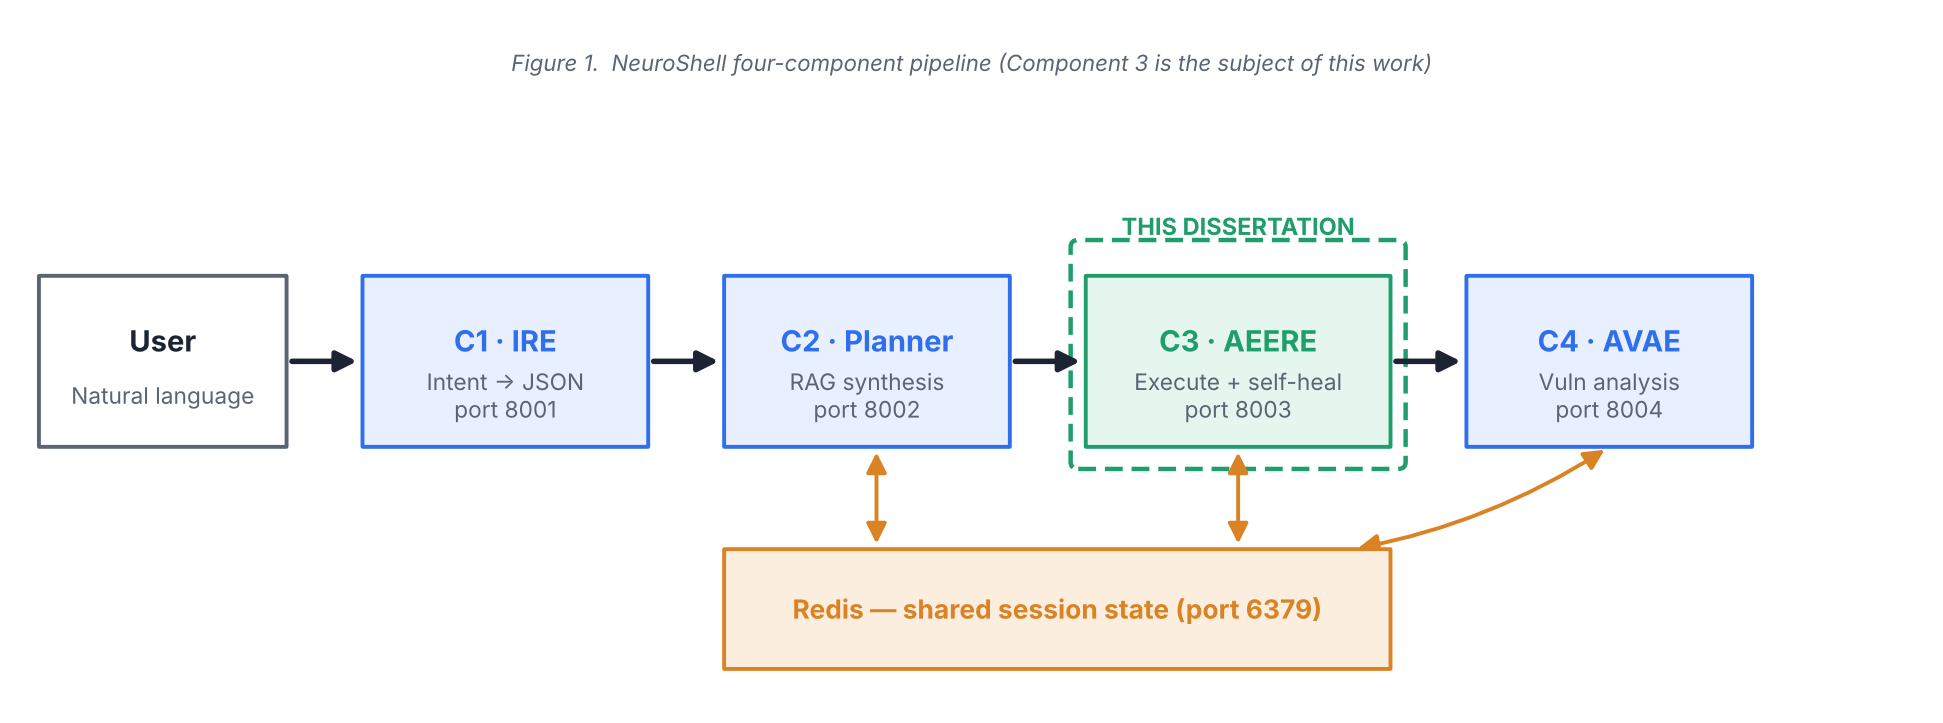
\includegraphics[width=0.92\textwidth]{C-03-Adoptive executer and error Recovery engine/vertopal_05e97fad080746c9b767567e93f99da6/media/image1.png}
  \caption{The four parts of NeuroShell (Component 3, the AEERE, is the subject
  of one of the component reports).}\label{fig:fourchain}
\end{figure}

The framework is organised as a group project (R26-CS-018) in which four
students each designed, implemented, and evaluated one component. The components
communicate over HTTP through FastAPI endpoints (ports 8001--8004) and share
state through Redis, so that each stage receives a well-defined structured
payload and produces a structured result. Separating the stages gives each
component an explicit input contract and provides a basis for checking whether
the information produced by one stage is preserved by the next.

\subsection{The Intent Recognition Engine (Component 1)}\label{sec:ctx-ire}

The IRE addresses the first gap in the chain: translating a free-form security
request into a validated, machine-readable intent contract. Large language
models (LLMs) are increasingly used to translate natural-language security
requests into machine-executable actions, but their stochastic output can
contain malformed structures, hallucinated parameters, out-of-scope targets, and
adversarial content, creating safety risks when connected to automated security
tools~\cite{deng2024pentestgpt}.

The IRE combines an offline, CPU-based language model with a multi-stage
pipeline and deterministic validation. The design constrains the raw output of
the model before any downstream dispatch: a guarded natural-language-understanding
gateway that accepts schema-valid, authorised, and in-scope intent contracts only.
The engine supports four security tools (Nmap, Gobuster, Nikto, and Nuclei) across
nine intent classes and is evaluated on 1,500 records with two offline backends
(Gemma and Qwen). Its closed trust boundary means no request text leaves the
device at inference time~\cite{liu2023promptinjection,nistairmf2023}.

\subsection{The Dynamic Planner and RAG Engine (Component 2)}\label{sec:ctx-planner}

Recognising a task does not, by itself, establish how that task should be
performed. The Dynamic Planner and Retrieval-Augmented Generation Engine
(Component~2) addresses the transition from a structured cybersecurity task to a
command-line instruction: it must select a suitable tool, preserve the supplied
target and operational parameters, and express the requested behaviour using the
syntax supported by that tool.

The component combines structured intent processing with retrieval of relevant
tool documentation. The knowledge base contains documentation and usage
information for the supported tools (Nmap, Nikto, and Gobuster). During planning,
relevant passages are retrieved and supplied as context for command synthesis,
so the generation stage has an explicit reference for tool options and usage
while the documentation collection is maintained separately from the language
model. Command correctness is treated as having several dimensions: a command may
use valid syntax while performing a different operation, or it may reflect the
intended operation while containing an unsupported argument. Evaluating syntax
alone therefore provides an incomplete assessment of the planner's
reliability~\cite{lewis2020rag,reimers2019sentencebert}.

\subsection{The Adaptive Execution and Error-Recovery Engine (Component 3)}\label{sec:ctx-aeere}

Security testers use a long list of command-line tools on Kali Linux, and these
tools fail very often: a tool may not be installed, a permission may be missing,
a target may be unreachable, or a command may use a wrong flag. When this
happens, conventional automated scans simply stop and wait. Even newer AI tools
such as PentestGPT, VulnBot, and xOffense do the same thing: they show the error
to the user and give up~\cite{pentestgpt,deng2024pentestgpt,vulnbot2025,xoffense2025}.

The Adaptive Execution and Error-Recovery Engine (AEERE, Component~3) addresses
this failure. Every command runs inside a Docker container with Kali Linux, so
nothing can harm the real computer. If the command fails, the engine reads the
error, works out what went wrong, fixes the command, and tries again, all by
itself. To work out what went wrong, it uses three steps one after another: a
fast pattern check, a text-similarity check, and finally a local AI model (Gemma,
run through Ollama) that reasons about the error. Before any fixed command is
allowed to run, it must pass three safety checks. Because the AI runs on the
same computer, no command, error, or target is ever sent to the
internet~\cite{yao2023react,shinn2023reflexion,gou2024critic}.

\subsection{The AI-Driven Vulnerability Analysis Engine (Component 4)}\label{sec:ctx-avae}

Automated security tools generate extensive vulnerability information that
needs manual interpretation and prioritisation. Traditional severity-based
approaches, particularly the Common Vulnerability Scoring System (CVSS), do not
by themselves establish whether a vulnerability has been exploited in the
real world. The AI-Driven Vulnerability Analysis Engine (AVAE, Component~4) is
responsible for transforming raw security assessment outputs into structured and
prioritised vulnerability information.

The component receives execution results from the AEERE through a structured
JSON interface and processes outputs of Nmap, Nikto, and Gobuster using dedicated
parsing mechanisms. It extracts IP addresses, open ports, running services, CVE
identifiers, and discovered web paths, and enriches them with vulnerability
intelligence from the National Vulnerability Database (NVD), the CISA Known
Exploited Vulnerabilities (KEV) catalogue, and the Exploit Prediction Scoring
System (EPSS). A central contribution is an Extreme Gradient Boosting (XGBoost)
classifier that uses five features (CVSS v3 score, EPSS score, EPSS percentile,
vulnerability age, and an engineered CVSS--EPSS interaction) to identify
vulnerabilities associated with documented exploitation evidence, with SHapley
Additive exPlanations (SHAP) providing interpretability. Neo4j graph-based
storage maintains relationships between sessions, hosts, services, and
vulnerabilities~\cite{bozorgi2010beyond,sabottke2015vulnerability,lundberg2017shap,
chen2016xgboost,jacobs2023epss}.

\subsection{Comparison with Existing Systems}\label{sec:existing}

Research on LLMs in penetration testing has demonstrated their potential to
support tool use, interpret execution output, and propose subsequent actions.
PentestGPT investigates these capabilities within a broader penetration-testing
workflow and identifies difficulties in maintaining the context of an entire
testing scenario~\cite{deng2024pentestgpt}; it relies on cloud-hosted GPT-class
models and offers no autonomous error-recovery loop. ReAct and Reflexion
demonstrate reasoning-acting and verbal self-reflection patterns for agents, and
CRITIC implements tool-interactive self-correction, but none of these is
specialised for security-tool failure recovery or operates fully
offline~\cite{yao2023react,shinn2023reflexion,gou2024critic}. AutoAttacker,
VulnBot, and xOffense move closer to autonomous offensive operations, yet they
depend on remote models and still stop on tool
failure~\cite{autoattacker2024,vulnbot2025,xoffense2025}. RepairAgent and SCoRe
target program repair rather than penetration-testing tool chains
~\cite{repairagent2024,score2024}. NL2Bash and related work show that
natural-language-to-shell translation is feasible but do not integrate intent
guarding, sandboxed execution, or vulnerability analysis~\cite{nl2bash2018}.

The NeuroShell framework differs from each of these categories in at least one
respect. Unlike generation-side copilots, it guards every intent with
deterministic validation. Unlike tool-integration work, it grounds command
synthesis in a maintainable documentation knowledge base. Unlike execution
frameworks that stop on failure, it autonomously recovers tool errors inside a
sandbox. And unlike cloud-hosted analysis pipelines, it runs all model inference
locally, which is a structural difference for air-gapped and regulated
deployments. \cref{tab:existing-chart} summarises this positioning.

\begin{table}[htbp]
  \centering
  \begin{tabular}{@{}p{0.26\textwidth}p{0.70\textwidth}@{}}
    \toprule
    \textbf{Category} & \textbf{Limitation addressed by NeuroShell}\\
    \midrule
    Deterministic tooling (Nmap, Metasploit) & No natural-language interface; no analysis of intent safety.\\
    Generation-side copilots (PentestGPT) & No deterministic intent guarding; cloud-hosted; no error recovery.\\
    Tool-integration techniques (ReAct, CRITIC) & Not security-specific; no sandboxed execution chain.\\
    Autonomous offensive agents (VulnBot, xOffense) & Stop on tool failure; remote models; no vulnerability prioritisation.\\
    Repair/self-correction (RepairAgent, SCoRe) & Target program repair, not security-tool failure recovery.\\
    \bottomrule
  \end{tabular}
  \caption{Positioning of NeuroShell against existing system categories.}\label{tab:existing-chart}
\end{table}

\subsection{Conceptual Framework and Design Principles}\label{sec:conceptual}

The combined design rests on a small set of principles that recur in every
component. First, \emph{boundary over intent}: the framework prefers to state,
enforce, and verify its boundaries (schema, scope, authorisation, sandbox)
rather than to rely on the model's good behaviour. Second, \emph{structured
contracts}: each stage communicates through a validated, machine-readable
payload (intent contract, planner output, execution result, analysis output)
rather than prose. Third, \emph{guarded autonomy}: the framework automates the
intent-to-command-to-report chain, but every automatically generated artefact
must pass a deterministic predicate before it is used. Fourth, \emph{closed
trust boundary}: all model inference is local, and no operational text leaves
the deployment machine.

\begin{figure}[htbp]
  \centering
  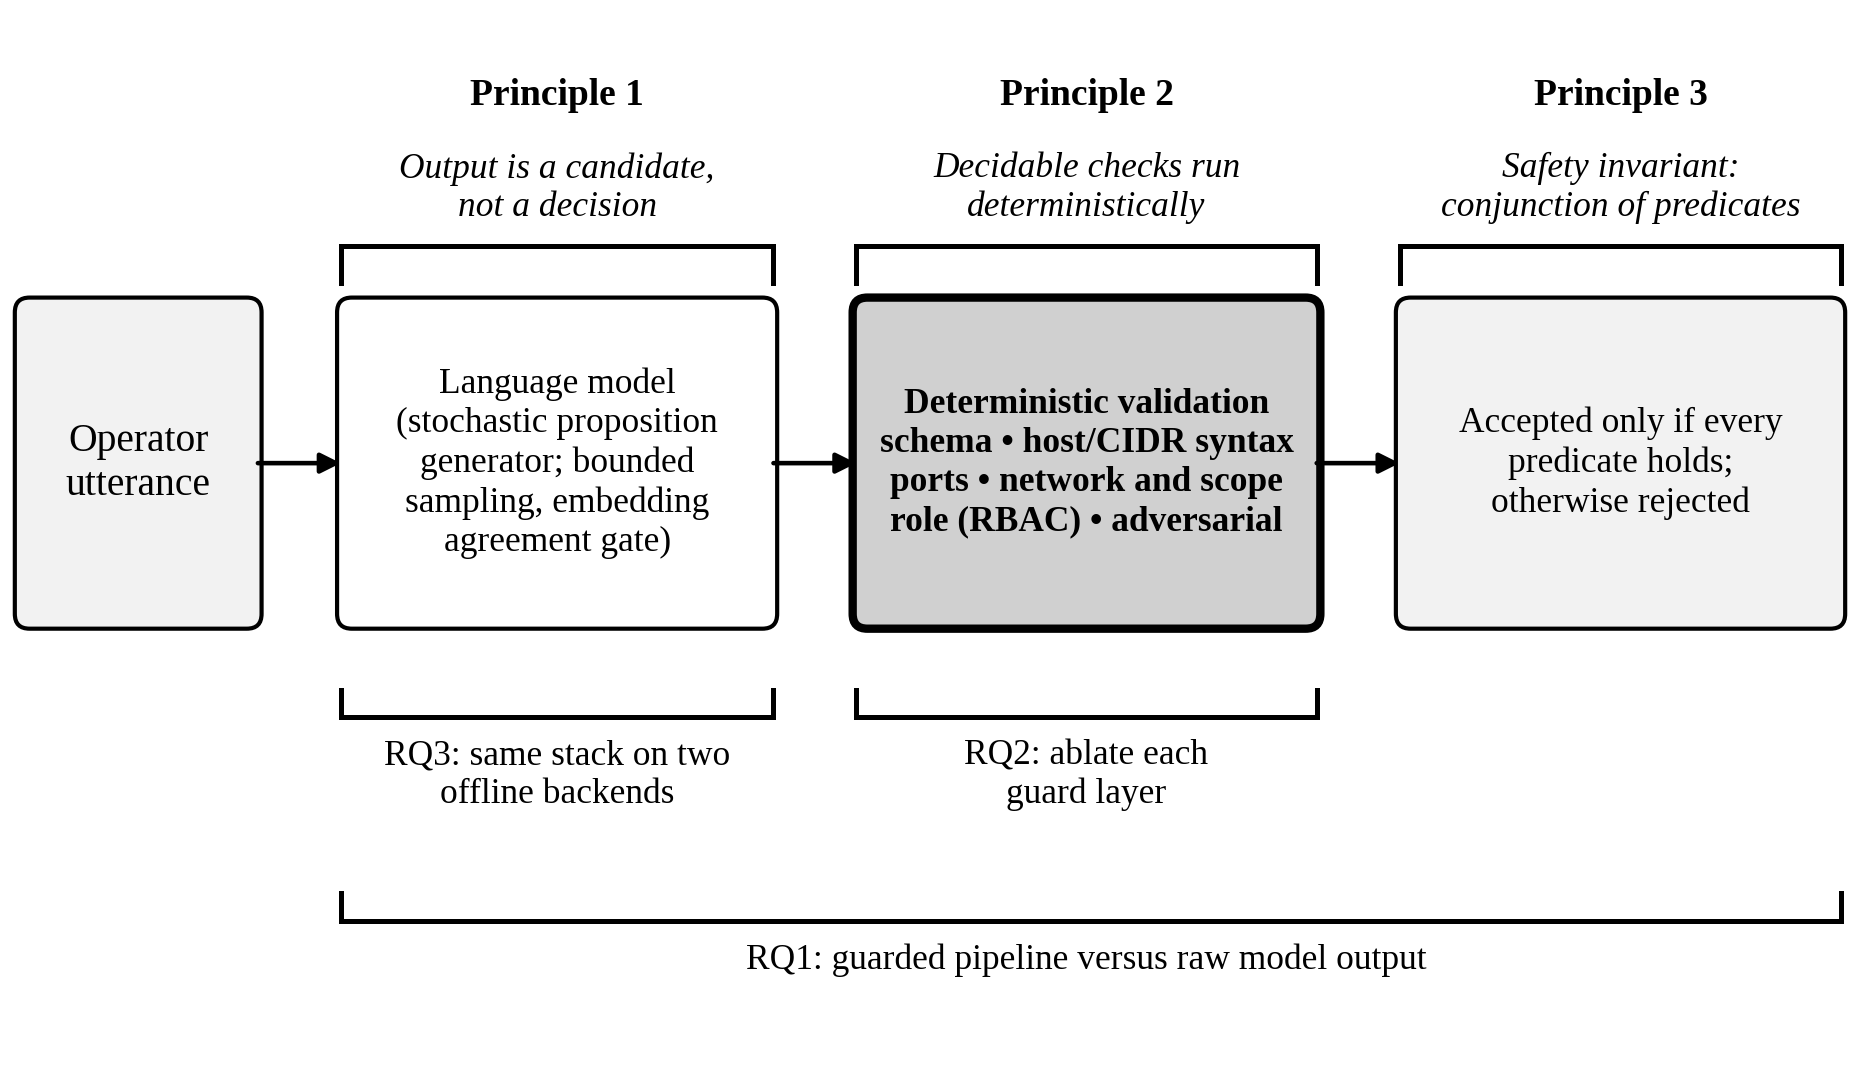
\includegraphics[width=0.9\textwidth]{C-01-Intetrecodnition Engine.pdf/vertopal_433ccb30063e47f1ba4c32a79683aeea/media/image3.png}
  \caption{Conceptual framework of the IRE within the NeuroShell chain: from the
  request to the guarded intent contract that downstream components consume.}\label{fig:conceptual}
\end{figure}

These principles enter the design formally. The IRE defines a guarded decision
function \(\Phi\) over the input utterance \(x\), and the safety invariant that
an intent is accepted only when the conjunction of the deterministic predicates
holds:
\[
  \mathit{Accepted}\bigl(\Phi(x)\bigr)\;\Longrightarrow\;
  \bigwedge_{k \in K} P_{k}(x),
  \qquad K=\{S5,S6,S6B,S7,\mathrm{RBAC},M1\},
\]
where each \(P_k\) is a deterministic predicate (schema, regex, network,
scope, authorisation, and adversarial-input checks) that is recomputed without
further model calls. The same safety-by-predicate attitude appears in the
planner's validation and safety filters, the AEERE's three checks applied to
every fixed command, and the AVAE's feature-grounded scoring.

\section{Research Gap}\label{sec:gap}

\subsection{Gaps in Offensive-Security Automation}\label{sec:gap-overall}

The literature is consistent on several limitations. First, existing AI security
copilots execute a plan but do not fix their own failures; an error message
terminates the run and requires human intervention. Second, most systems accept
natural language directly and pass model output to tools without a deterministic
safety boundary, so malformed, out-of-scope or adversarial content can reach a
live tool. Third, tool documentation is either embedded in the prompt or
unavailable, and command generation is not grounded in an explicit,
maintainable reference. Fourth, when findings are produced, they are typically
raw tool output: vulnerability intelligence is not combined with machine-learning
classification to prioritise what should be reviewed first. Fifth, almost all of
the surveyed systems rely on cloud-hosted models, which conflicts with
organisations whose policies require that commands, errors, and targets never
leave the premises.

\subsection{Gap Specific to Each Component}\label{sec:gap-percomponent}

For the IRE, the gap is the absence of a small, offline model combined with
deterministic validation to gate a security copilot; existing research either
uses unguarded output or relies on remote model safety. For the planner, the gap
is the translation of an explicit structured intent into a validated command,
grounded in documentation and checked against explicit validation and safety
constraints. For the AEERE, the gap is the handling of tool failure: no surveyed
system reads a failed security tool's error, labels it, and writes a fixed
command by itself, and none does so fully on the machine. For the AVAE, the gap
is integrating scanner-output parsing, vulnerability intelligence, an
exploitation-evidence classifier, and explainable prioritisation into a single
analysis workflow that operates within an autonomous assessment chain.

\section{Research Problem}\label{sec:problem}

\subsection{Framework Problem Statement}\label{sec:problem-overall}

The overarching problem addressed by this research is how to move from a
natural-language security request to an explainable, prioritised vulnerability
report with minimal human intervention, while keeping every step within a
controlled safety boundary. Concretely: how can a framework translate a request
into a validated intent, plan a grounded command, execute and recover that
command autonomously in a sandbox, and finally analyse the results, such that no
insecure operation is ever emitted and no operational data leaves the local
environment?

\subsection{Problem Specific to Each Component}\label{sec:problem-percomponent}

Each component addresses a distinct sub-problem. The IRE must translate
free-form instructions into validated intent contracts while rejecting
malformed, hallucinated, out-of-scope, and adversarial utterances. The planner
must translate a structured cybersecurity intent into a command that accurately
represents the requested operation and satisfies the constraints of the
supported tool environment, preserving target and parameters through
generation. The AEERE must read a failed security tool's error, understand it,
and write a fixed command by itself, with no human help, under a sandbox and
safety policy. The AVAE must process security assessment outputs and prioritise
vulnerabilities using exploitation evidence while keeping predictions
explainable.

\section{Research Objectives}\label{sec:objectives}

\subsection{Main Objective}\label{sec:objectives-main}

The main objective of this research is to design, develop, and evaluate
NeuroShell, an autonomous natural-language-driven orchestration framework for
offensive security operations, in which four cooperating components convert a
natural-language request into validated intents, grounded commands, sandboxed
execution with autonomous error recovery, and explainable vulnerability
prioritisation---with all model inference performed locally.

\subsection{Specific Objectives per Component}\label{sec:objectives-specific}

The following specific objectives were established across the four components:

\begin{enumerate}
  \item To design a guarded intent-recognition pipeline that combines an offline
  language model with deterministic validation, and to author an annotated
  evaluation data set covering well-formed and deliberately flawed prompt
  categories, along with an evaluation harness and a per-layer ablation
  protocol (IRE).
  \item To design a planning workflow that processes the structured intent
  contract, to develop a retrievable knowledge base containing documentation for
  Nmap, Nikto, and Gobuster, to implement tool selection and
  documentation-grounded command synthesis, and to implement validation and
  safety checks over generated commands, exposed through an API (planner).
  \item To design and implement a sandboxed execution engine with a five-stage
  error-recovery loop, a three-step fast-to-slow error-labelling cascade that
  ends in a local AI model, an eight-type Kali-specific error list with
  retry limits and tool-swap rules, and three safety checks applied to every
  fixed command (AEERE).
  \item To prepare a structured vulnerability-intelligence data set, to develop
  scanner-output parsers for Nmap, Nikto, and Gobuster, to train and evaluate an
  XGBoost classifier using five vulnerability features, and to implement
  SHAP-based explainability, contextual prioritisation, Neo4j graph storage, and
  a FastAPI interface (AVAE).
\end{enumerate}

\subsection{Research Questions}\label{sec:rqs}

The component reports define research questions aligned with these objectives:

\begin{enumerate}
  \item \textbf{IRE:} Does a guarded, offline-language-model pipeline produce
  schema-valid, authorised, and in-scope intent contracts more reliably than raw
  model output, and which pipeline stage contributes most to safety?
  \item \textbf{Planner:} How accurately does the planner translate structured
  intents into commands that select the appropriate tool, preserve the supplied
  parameters, and use valid syntax; what effect does retrieval have on command
  correctness and latency; and how effectively do the validation and safety
  mechanisms reject invalid requests?
  \item \textbf{AEERE:} Can a system read a failed security tool's error,
  label it, and produce a fixed command by itself, and can it do so fast enough
  and without ever letting a dangerous command through?
  \item \textbf{AVAE:} How effectively can vulnerability-intelligence features
  support classification of vulnerabilities according to known exploitation
  evidence using XGBoost, and how well can SHAP explanations support
  interpretation and prioritisation?
\end{enumerate}

\section{Scope, Limitations and Assumptions}\label{sec:scope}

The framework is scoped to a defined tool set and a defined trust boundary. The
planner and the parsers support Nmap, Nikto, and Gobuster; the IRE supports these
three tools plus Nuclei. The AEERE builds and tests on a data set of 8,000
labelled Kali command-failure cases covering ten error types, more than eighteen
tools, and three difficulty levels. The AVAE builds its classifier on a
curated data set of 155,852 vulnerability records derived from public
vulnerability sources, with the classification target defined from CISA KEV
membership. All model inference is performed locally through Ollama; no command,
error text, or target is transmitted off the deployment machine.

Several limitations bound the generality of the results. Natural-language intent
recognition is the responsibility of Component~1; the planner consumes the
resulting structured contract rather than performing the complete
interpretation of the original request. Findings for the planner are limited to
the supported tools, documented options, and cases included in the evaluation.
The AEERE's data set is hand-built, so real-world terminal errors may behave
differently. The AVAE model relies on five structured features and a
KEV-derived target, so its predictions reflect relationships within the
available data. Most evaluation data are single-run point estimates obtained on
limited hardware, and no component completed a formal user or stakeholder
validation study. The framework assumes that all test targets are private,
RFC-1918 lab addresses that cannot reach any real system.

\section{Thesis Structure}\label{sec:structure}

This combined dissertation is organised into four chapters. \cref{ch:methodology}
presents the research methodology and the design of the framework, including the
research approach, the architecture, the ethical and safety measures, the
commercialisation aspects, and the testing and implementation strategy.
\cref{ch:results} reports the results and findings of each component, together
with a discussion and a summary of each student's contribution.
\cref{ch:conclusions} concludes the study, assesses the achievement of the
objectives, and identifies recommendations and future work. The appendices
provide the research instruments used by each component and the disclosure of
AI usage.